Database designet er en to delt affære. Der er selve strukturen i databasen også er der koden som tilgår databasen.
Disse beskrive begge i følgende afsnit.

\subsubsection{Database Opbygning}
Opbygningen af den fysiske database er sket ved at opstille designet via et DS diagram som kan ses på figur \ref{fig:DSD} og derefter sætte den op med SQL Serber Database Project fra visual Studio. 

\begin{figure}[H]
    \centering
    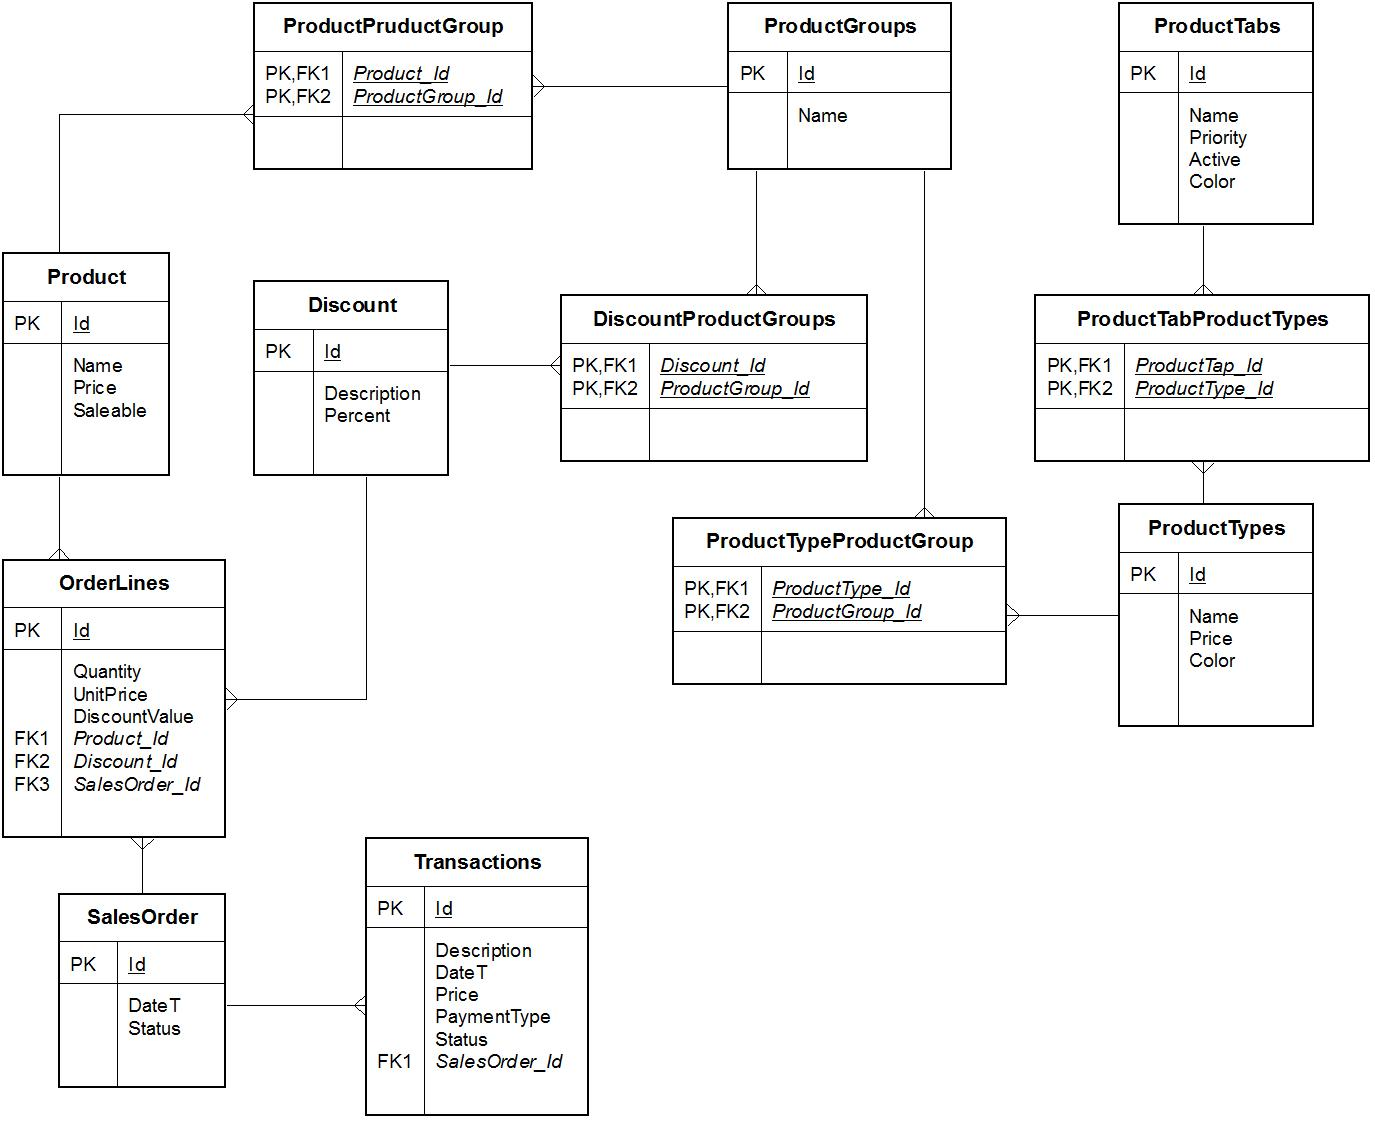
\includegraphics[width=0.6\textwidth]{N+1/DataView/DabDSD}
    \caption{Data Structure Diagram over databasen}
    \label{fig:DSD}
\end{figure}
Databasen er lavet så det er muligt at have flere salgsbestillinger under et salg og et salg skal kunne betales med flere Transaktioner, disse er lavet ved at opsætte nogle one-to-many og many-to-many forhold, som der kan læses nærmere om under DataView i dokumentationen.
\newline
\newline
som det kan ses består OrderLine i databasen af alle de informationer en salgsbestilling kan bestå af, som vare, rabat og antallet af vare. mange af disse har deres egene tabeller så varer og rabatter også kan have nogle fast defineret værdier.
\newline
\newline
Som det kan ses på figur \ref{fig:DSD}, har den tabellerne Product, ProductGroup, ProductType og ProductTab. Dette design er lavet for at kunne give nogle større grupper rabat. ProductTaps er lavet i forhold til GUI'en så man nemt kunne få alle de vare der skulle stå på hver Taps ind.  


\subsubsection{Database kode}
For at kunne tilgå databasen fra C\# blev det besluttet at bruge \gls{EF}. 
Det blev valgt at bruge "Code First from existing database" da designet af databasen var lavet i forvejen.
Ved at følge den fremgangsmåde bliver der lavet en model af databasen i form af objekter som \gls{EF} 
kan mappe til i figur \ref{fig:CodeFirstFromDB} er princippet illustreret.

\begin{figure}[H]
    \centering
	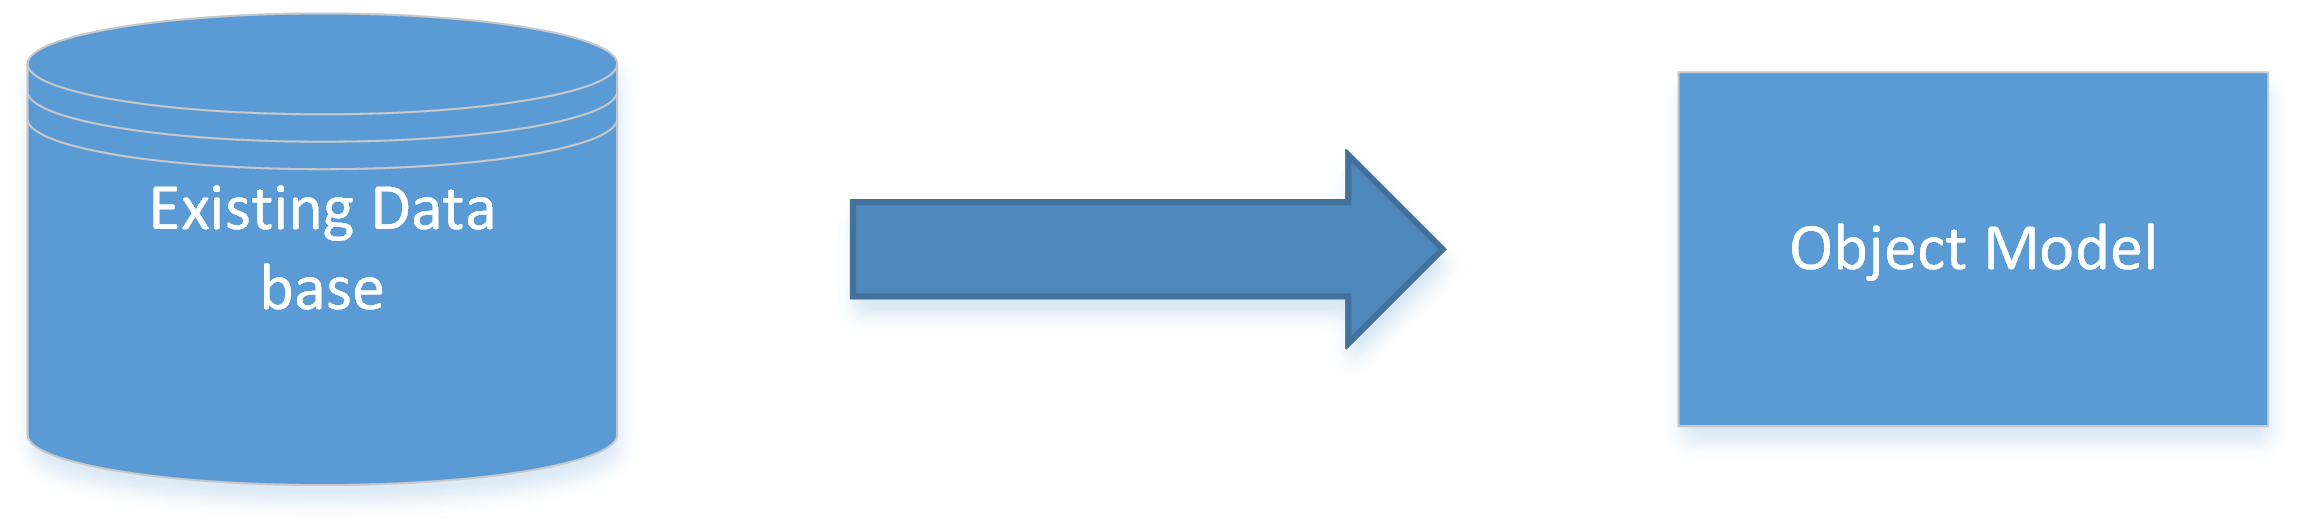
\includegraphics[scale=1]{Rapport/EFCFFDB.PNG}
	\caption{Skitse af GUI}
	\label{fig:CodeFirstFromDB}
\end{figure} 

Det virkede meget godt til første iteration af databasen, men herefter viste det sig at være lettere at få \gls{EF} til at bygge
databasen udfra koden ved ændringer.
\newline
Det blev også besluttet at pakke \gls{EF} ind i \gls{DAL} dette blev brugt for at skille framework koden fra vores program.
\gls{DAL} Består af tre klasser en Facade klasse, en Unitofwork klasse og en Repository klasse. 
Facaden er brugt til at sørge for at der kun findes et Unitofwork af gangen. 
Unitofwork er en samling af Repositorys, Unitofwork's opgave er at sørge for at der bliver kaldt "Save" på \gls{EF}'s context.
Repository er metoder til at udføre Create, Read, Update and Delete.
